% !TeX spellcheck = es_ES
% !TeX root = ../metalurgy.tex
\part{Aceros inoxidables}

% \includegraphics{schaeffler.png}

\begin{figure}[htb]
	\centering
	\includegraphics[width=0.6\linewidth]{fig/schaeffler.png}
	\caption{Diagrama de Schaeffler.}
	\label{fig:schaeffler}
\end{figure}



Grupo de aceros de alta aleación diseñados para tener resistencia a la corrosión en un amplio rango de servicio y alta resistencia en un rango amplio de temperaturas.

Las aplicaciones principales de estos aceros son en plantas generadoras de energía, centrales hidráulicas, plantas petroquímicas, industria farmacéutica, piezas de maquinas, arquitectura (decoración), aplicaciones marítimas.

Se pueden clasificar en dos tipos principales
\begin{description}
	\item[Austeníticos] Son los aceros inoxidables de mayor uso debido a la combinación de sus propiedades mecánicas y su alta resistencia a la corrosión
	\item[Ferríticos] Se usan mucho menos que los austeníticos pero poseen algunas ventajas como menor costo y mayor resistencia a la corrosión bajo tensión
	\item[Martensíticos] Son los de mayor resistencia mecánica pero menor resistencia a la corrosión
	\item[Duplex o austenoferríticos] Son el tercer grupo más utilizado , poseen buena combinación de propiedades mecánicas y resistencia a la corrosión
	\item[Endurecibles por precipitación] Comprenden a los Austeníticos, semiausteníticos y martensíticos  
\end{description}

\section{Corrosión}
Deterioro de un material por la acción química del medio que lo rodea. A excepción de los nobles, los metales son termodinámicamente inestables al contacto con el aire y forman óxidos. Si la reacción es ``lenta"{} (desde un punto de vista cinético) la corrosión puede llegar a aceptarse. Si es ``rápida"{} y limita la vida del componenta surgen problemas de costo y fiabilidad mecánica.

\subsection{Clasificación}
\begin{description}
	\item[Generalizada] A nivel macroscópico, la superficie es atacada uniformemente. Es predecible y controlable. Se puede prevenir si se diseña con un sobre-espesor uniforme. El daño es proporcional a la cantidad de material removido.
	\item[Localizada] Daño localizado progresa rápido. Resulta difícil predecir, controlar y detectar. El daño puede ser muy grande aunque la cantidad de material sea mínima. Es muy problemático. A continuación se tienen 4 tipos de corrosión localizada:
	      \begin{description}
		      \item[Picado/Pitting] Promovido por la presencia de iones $Cl^{-1}$, alta temperatura y baja velocidad de circulación del fluido. Si la capa pasivante se rompe localmente y no se forma rápido otra la corrosión avanza y se genera pozos en forma de túneles que pueden perforar el material en corto tiempo aumentando el riesgo de avance de fisura por fatiga. El Cromo, Molibdeno y nitrógeno aumentan la resistencia al picado según el \textbf{índice de picado}: $IP=\% \textrm{Cr} + 3,3\% \textrm{Mo} + X \%\textrm{N}$,  donde $X$ es 0\footnote{El nitrógeno es prácticamente insoluble en la ferrita a temperatura ambiente.}, 16 o 30 para inoxidables ferríticos, duplex o austeníticos, respectivamente. 
		      \item[Rendijas] Se da en zonas donde el fluido no llega a circular debido a la geometría/orientación de la pieza. Cuando se consume el oxigeno se forma una \textbf{celda de aereación diferencial} entre la rendija y el resto de la superficie metálica. Evitable con buen diseño de pieza, reduciendo iones de cloro y reduciendo la temperatura. El Molibdeno mejora la resistencia ante este tipo de corrosión.
		      \item[Bajo tensión] Puede dar lugar  fallas catastróficas a partir de fisuración provocada por la combinación del \textbf{medio} y \textbf{tensión de tracción}. Em general la fisura rompe por fractura frágil. Los aceros inoxidables austeníticos y martensiticos son los más susceptibles. Los aceros austeníticos y martensíticos son los más susceptibles. Hay dos tipos de SCC (Stress  corrosión cracking) más conocidos
		      \begin{description}
				  \item[SCC Fisuración transgranular ramificada] Producido por soluciones con \textbf{cloruros} a temperatura mayor a 60\grad. Agravado por mayor cantidad de cloruros, deformación plástica previa, mayor temperatura y un pH entre 3 y 8.
				  \item[SCC Fisuración intergranular] Causado por soluciones cáusticas de no menos de 20\% concentración a alta temperatura (>130\grad)
			  \end{description}
		      \item[Granular] Asociada a fenómeno de precipitación de carburos ricos en Cr en los bordes de grano de las microestructuras.
	      \end{description}
\end{description}


\subsection{Pasividad}
La pasivación de un metal se refiere a la formación de una delgada capa de óxido al ser sometido a un diferencial de potencial ($\Delta V$) mayor al potencial de pasivación. Esta capa aísla al metal del medio y hace que disminuya la velocidad de corrosión en varios ordenes de magnitud. Para que sea efectiva la capa esta debe ser fina, continua, no porosa, insoluble en el medio, y debe poder regenerarse rápidamente al ser dañada (ralladura, mecanizado). 

El aluminio, por ejemplo, no es electronegativo pero es fuertemente pasivado. El hierro puede pasivarse pero a un alto $\Delta V$. La inclusión de cromo (Cr) en un 12\% o más hace que el metal pueda oxidarse fácil

\subsubsection*{Variables en la estabilidad de la capa pasivante}
\begin{description}
	\item[Composición química del acero] Factor principal es el contenido de Cr (12\% mínimo) para pasivar con soluciones acuosas neutras. En general la heterogeneidades (segregaciones, precip. de carburos) hacen que disminuya la estabilidad.
	\item[Composición del medio] Los inoxidables se pasivan solo cuando el medio es altamente oxidante (acuosos, $HNO_3$). La presencia de iones de halógenos (CL$^{-1}$) desestabilizan la capa pasivante generando corrosión localizada y son es la principal razón por fallas. Un medio básico (pH alto) es más estabilizante para una capa pasivante.
	\item[Variables operativas] En general, la resistencia a la corrosión disminuye con el aumento de la temperatura. La velocidad relativa entre el medio y la superficie afecta la formación de la capa. A mayor velocidad hay mayor aporte de $O_2$, aumentando la velocidad de oxidación y estabilidad de la capa (mientras que no haya fenomeno de erosión--corrosión). Una velocidad alta de circulación puede también prevenir que decanten partículas que catalizen la corrosión.
	\item[Factores de diseño] La presencia de rendijas o alta rugosidad crean zonas que favorecen la oxidación localizada.
\end{description}

\section{Aceros inoxidables austeníticos}
Se trata del grupo de aceros inoxidables que mejor combina propiedades mecánicas y tecnologías con resistencia a la corrosión a precio razonable. Constituyen 70\% de la producción total de aceros inoxidables. 



El Cromo es un elemento alfágeno y consecuentemente no podrían existir aceros inoxidables austeníticos con Cr solamente. Es necesario recurrir a un elemento \textbf{gamágeno}. La composición típica de un acero austenítico inoxidable :
\begin{description}
	\item[Cr] 16 a 30\%
	\item[Ni] 8 a 30\%
	\item[Mo] Hasta 4\%
	\item[Mn] $\approx$ 2\%
	\item[C] Menor de 0,1\%
\end{description}

\subsection{Ventajas de una estructura FCC}
El costo de obtener un acero inoxidable austenítico puede ser justificado según
\begin{itemize}
	\item La gran ductilidad y baja tensión de fluencia por poseer 12 sistemas de deslizamiento. Se traduce en una alta capacidad para el conformado plástico, especialmente en frío.
	\item Los metales monofásicos FCC no poseen \Tdf~ (transición dúctil-frágil) y además poseen alta tenacidad, la cual conservan a hasta bajas temperaturas ideal para aplicaciones criogénicas.
	\item Estructura FCC es inherentemente más resistente a la fluencia a alta temperatura (creep) debido a la menor energía de falla de apilamiento comparado a estructura BCC.
	\item Intersticiales tienen mayor solubilidad y menor difusividad. Esto ralentiza la precipitación de carburos ricos en Cr y en ciertas condiciones lo evita. Estos carburos deterioran la resistencia a la corrosión como veremos
	\item En sistema Fe-Ni-Cr la estructura FCC es amagnética.
\end{itemize}



\subsection{Elección de gamágeno}
El Cr es un elemento alfágeno, entonces se necesita de un gamágeno para estabilizar la austenita a temperatura ambiente.
\begin{description}
	\item[C] Debe ser bajo porque favorece la precipitación de carburos de Cr, lo cual favorece la corrosión
	\item[N] No se usa ya que no estabiliza la austenita hasta bajas temperaturas
	\item[Mn] Se usa en casi todos los austeníticos pero no es el gamágeno principal. Estabiliza la austenita a temperatura ambiente pero no baja tanto $M_s$. La austenita rica en Mn no posee tan buenas propiedades mecánicas como el sistema Fe-Ni.
	\item[Ni] Estabiliza austenita hasta bajas temperaturas. Baja la $M_s$ (reduciendo la formación de martensita, cosa indeseable), mejora la tenacidad y aumenta la resistencia a la corrosión. A mayor cantidad de Cr, Mo y otros alfágenos se requiere de mayor Ni para balancear la estructura y lograr que sea austenítica. La desventaja principal es su \textbf{costo} elevado.
\end{description}

El acero inoxidable en el cual todos los demás están basados tiene la composición 18\% Cr -- 8\% N -- 0,15\% C y algo de Mn. A temperatura ambiente este acero tendría una estructura parcialmente austenítica con algo de ferrita y además carburos de Cromo. La austenita no transforma a martensita pues la $M_s$ es muy baja a consecuencia del contenido de aleantes, en particular el Ni.

A temperatura ambiente un acero inoxidable austenítico contiene muy poca martensita por el $M_s$ bajo, poca ferrita y algunos carburos.

\subsection{Precipitación de carburos de Cromo}
\label{ssec:sensibilizacion}
El \%C aumenta la temperatura a la cual precipitan los carburos del Cromo y la acelera. Los carburos de Cromo nuclean en los borde de grano y bordes de maclas de la austenita. Alrededor de los carburos queda una zona empobrecida en Cr, lo cual lleva a la \textbf{sensibilización}. El impacto se debe al alto contenido de Cromo por carburo M$_{23}$C$_6$ (+70\% en peso).

La sensibilización da origen a la \textbf{corrosión intergranular} y ocurre frecuentemente en aceros austeníticos ya que cuando hay un proceso de alta temperatura el carbono se disuelve y re-precipita al enfriarse.
ralentiza. 

\subsubsection{Causas}
Cualquier proceso que someta al acero a altas temperaturas y posteriormente \textbf{no lo enfrie suficientemente rápido} como para evitar la precipitación de carburos de Cromo, conducirá a un estado sensibilizado. El grado de sensibilización dependerá del contenido de C del acero y la velocidad de enfriamiento.

\begin{itemize}
	\item Soldadura
	\item Tratamientos térmicos
	\item Solidificación
	\item Conformado en caliente
\end{itemize}

\subsubsection{Métodos para revertir la sensibilización}

\begin{description}
	\item[Temple de solución o Hipertemple] Temperatura entre 1010 y 1120\grad y luego un medio de enfriamiento que aporte la velocidad necesaria para prevenir precipitación de carburos de Cr. Limitado por espesor de pieza y distorsión permisible
\end{description}


\subsubsection{Métodos para prevenir la sensibilización}

\begin{description}
	\item[Disminución de \%C]  Grados de aceros 304L, 316L de bajo C ($\leq0,03\%$C) tienen un efecto notable comparado a sus contrapartes 304 y 316 ($\approx 0,08\%$C). La disminución del C retrasa la precipitación y disminuyen su cantidad. Bajo ciertas condiciones estos grados pueden ser soldados sin necesidad de un tratamiento de temple de solubilización posterior. Por otro lado la disminución del C permite aplicar el temple de solución facilmente si fuera necesario. Muy usado en piezas de alto grosor. 
	\item[Agregado de elementos estabilizadores] Nb, Ti, Ta. Grados \textbf{AISI 321, 347 y 348}. Estos elementos forman carburos facilmente y compiten con el Cr, así disminuyendo o evitando la precipitación de carburos de Cr. Para algunos grados se aplica un \textbf{tratamiento de estabilización} en el cual se calienta el acero en un rango de temperatura donde precipitan los carburos de los elementos estabilizadores y en cam,bio es lenta la precipitación de los carburos de Cr (850-900\grad varias horas)
	\item[Composición química] La composición química de estos aceros posee una cantidad de Cr no menor al 16\%. A medida que se agrega Cr, o bien se agrega Mo, se mejora la resistencia a la corrosión y sensibilización. Sin embargo esto debe compensarse con una cantidad adecuada de Ni para poder obtener una estructura austenítica minimizando la presencia de ferrita $\delta$. El \textbf{C} se debe mantener bajo (usualmente <0,08\%) para disminuir la sensibilización. Los grados de bajo C poseen un máximo de 0,03\%. El \textbf{Ti, Nb y Ta} se usan en pequeñas proporciones como estabilizadores en algunos grados. El \textbf{Al, Si y Cu} se agregan en ciertos grados especiales para aumentar la resistencia a algún tipo de corrosión u oxidación en caliente. El \textbf{Mn} está presente en todos los grados (aproximadamente en un 2\%)   
\end{description}

\subsection{Propiedades mecánicas}

\subsubsection{Endurecimiento}
A pesar de su baja tensión de fluencia, se puede decir que los aceros austeníticos presentan las mejor combinación de propiedades mecánicas. En estado de temple de solución, los aceros austeníticos tienen una $\sigma_y$ entre \textbf{200 y 300MPa}, la cual es comparable a un acero común laminado en caliente de 0,1\% o 0,2\% C (AISI 1010, 1020). La tensión de fluencia es una gran desventaja pues los métodos de endurecimiento son restringidos pues no deben afectar demasiado a la resistencia a la corrosión.

El \textbf{refinamiento de grano} no es tan fácil de lograr como en aceros al carbono. No puede lograrse por tratamiento normalizado, pues no existe cambio alotrópico $\alpha \rightarrow \gamma$. Aplicando deformación en frío y luego un recocido se reduce el tamaño del grano apreciablemente. Surge un problema en este último tratamiento: el rango de temperaturas del recocido cae dentro del rango de precipitación de carburos de Cr. Por otra parte el \textbf{coeficiente $k_y$ de la ecuación Hall-Petch es aproximadamente la mitad que para aceros ferríticos} de modo que es menos efectiva la reducción en tamaño de grano que en aceros ferríticos de baja aleación.

El \textbf{endurecimiento por precipitación} se usa en algunos aceros inoxidables austeníticos, como así en semiausteníticos y martensíticos. Estos aceros austeníticos tienen mayor resistencia mecánica ($R_{p0,2}$ entre \textbf{500 y 900MPa}). En general el precipitado no involucra al Cr ni C, si no otro tipo \textbf{intermetálico}. De modos estos aceros tienen más problemas de fabricación (conformado/soldadura) que los austeníticos comunes y son más costosos de tratar térmicamente. Por todo esto su uso es más restringido que el austenítico inoxidable. 

Los aceros inoxidables austeníticos son principalmente \textbf{endurecidos por deformación en frío} debido a estos últimos puntos. El coeficiente de endurecimiento por deformación de estos aceros es muy alto pues poseen baja EFA.

En los aceros inoxidables austeníticos, durante la deformación plástica en frío se puede transformar algo de austentíta en martensita si es que la $M_d$ es suficientemente alta. La martensita eleva la resistencia y aumenta el coeficiente de endurecimiento por deformación. El elemento que más influye en esto es el Ni. Aceros con alto contenido de Ni poseen baja $M_d$ y se denominan \textbf{estables} ya que no transforma casi nada de austenita en martensita durante la deformación a temperatura ambiente. Otros aceros austeníticos inoxidables con menor cantidad de Ni presentan mayor transformación de martensita y se denominan \textbf{inestables.}

Dependiendo del proceso de conformado en frío, se puede desear un bajo coeficiente de endurecimiento por deformación (procesos de altas tensiones de compresión, ej. recalcado, laminación de roscas) o uno alto (procesos con tensiones uniaxiales o biaxiales). Un coeficiente bajo reduce el desgaste y el riesgo de rotura de la pieza durante el conformado. Hay grados diseñados espacialmente para presentar un alto coeficiente (AISI 301) y otros para lograr un coeficiente bajo (AISI 305 y 384).

Otro mecanismo de endurecimiento que se usa es el \textbf{endurecimiento por solución sólida}. Si se eligen los elementos adecuadamente, este mecanismo desmejora muy poco la resistencia a la corrosión y de hecho puede mejorarla. El principal endurecedor es el \textbf{Nitrogeno}. Este elemento endurece más que el C (50 contra 30MPa por cada 0,1\%), es más soluble que el C, aumenta la resistencia al picado y corrosión en rendijas, es menos nocivo que el C cuando precipita, al ser un poderoso gamágeno refuerza el efecto del Ni y Mn (el N es 20 veces más poderos que el Ni como gamágeno), el N baja la temperatura $M_s$ y $M_d$, y por último retrasa la precipitación de carburos M$_{23}$C$_{6}$. Ciertos grados usan el N como aleante importante.

\subsubsection{Ductilidad}
La ductilidad de los inoxidables austeníticos es excelente, en estado recocido el alargamiento porcentual (A\%) está entre 45 y 60\%, y la estricción (Z\%) está entre 50 y 70\%. 

Esta gran ductilidad combinada con un adecuado coeficiente de endurecimiento por deformación y una baja tensión de fluencia hace que sean muy conformables en todos los procesos de conformado en frío. Existen algunos feómenos de fragilización que deterioran la ductilidad (y aún más la tenacidad) que tienen que ver con la aparición de \textbf{fases intermetálicas}.

\subsubsection{Tenacidad}
En estado recocido la tenacidad de estos aceros es excelente y se mantiene en valores alto aún a muy bajas temperaturas. Por ende los aceros austeníticos inoxidables son muy usados en aplicaciones criogénicas (producción, transporte y almacenaje de gases líquidos).

La aparición de pequeñas cantidades de \textbf{fases intermetálicas fragilizan fuertemente al acero}. Debido a los tiempos necesarios para la aparición de estas fases, este tipo de fragilización es un tema de degradación del acero durante su servicio a altas temperaturas y no es de cuidado en la mayoría de los tratamientos térmicos a que se someten los aceros inoxidables austeníticos comunes.

La influencia de la precipitación de carburos M$_23$C$_6$ sobre la tenacidad depende de la cantidad de C del acero. A más C es mayor la cantidad de carburos precipitados durante la sensibilización y mayor su influencia en el \textbf{deterioro de la tenacidad}. Sin embaro, con excepción de los grados de muy alto C (por ejemplo el AISI 302 con 0,15\% max X), la tenacidad inicial de estos aceros es tan alta que aún en estado completamente sensibilizado se conserva un valor que es aceptable para muchas aplicaciones. 

Respecto de la incidencia de la \textbf{tranformación a martensita} a baja temperatura sobre la tenacidad se comprueba que, contrariamente a lo que se esperaría, no hay correlación entre la tenacidad a bajas temperaturas y el grado de estabilidad de la austenita de los diferentes grados de inoxidable austeníticos. De todos modos se debe recordar que la martensita que se produce en estos aceros es de muy bajo C y si bien presenta mayor resistencia mecánica que la austenita, su tenacidad no es muy baja.

\subsubsection{Fluencia lenta (creep)}

La estructura FCC es inherentemente más resistente a la fluencia lenta que la BCC pues posee mayor EFA. Debido a su excelente resistencia al creep, así como su alta resistencia a la oxidación en caliente y también ciertos tipos de corrosión de alta temperatura, los inoxidables austeníticos \textbf{son ampliamente usados como materiales de alta temperatura}. El Cr y el Mo en solución sólida aumentan la resistencia a la fluencia lenta, mientras que los carburos que forman el Nb y el Ti también hacen lo mismo cuando precipitan en forma fina y homogénea.

Los aceros inoxidables austeníticos solo presentan claras ventajas frente a aceros inox. martensíticos o de baja y media aleación al Cr, Cr--Mo, o Cr--Mo--V, a partir \textbf{de los 550\grad}. Esto se debe a que para temperaturas menores las tensiones admisibles que se usan en el diseño se basan en las propiedades de tracción a alta temperatura y no en las propiedades de fluencia lenta a alta temperatura.

Estos aceros también pueden sufrir de fenomenos de \textbf{precipitación de ciertas fases intermetálicas} que deterioran la ductilidad y tenacidad del acero y pueden conducir a fisuración o roturas durante las paradas y arranques en frío de las piezas.

\subsubsection{Formabilidad}
En estado recocido estos aceros tienen \textbf{muy buena formabilidad en frío}. \textbf{En cuanto a formabilidad en caliente}, los aceros inoxidables austeníticos, junto con las superaleaciones base Ni, presentan ciertas dificultades asociadas con su alto contenido de solutos, bajas temperaturas de sólidus, gran resistencia en caliente, precipitación de ciertas fases (ferrita $\delta$ y carburos) y un rango bastante amplio de tendencia a la \textbf{fisuración intergranular}. La presencia de ferrita $\delta$ deteriora fuertemente la ductilidad de estos aceros y en este sentido los elementos alfágenos (en especial el Mo) tienen gran influencia.


\subsubsection{Soldabilidad}

Los aceros inoxidable austeníticos son los de mejor soldabilidad entre los diferentes grupos de aceros inoxidables, sin embargo presentan dos problemas que son salvables con relativa facilidad.

\begin{description}
	\item[Sensibilización en la ZAC] Durante la soldadura por arco, una parte de la zona afectada por el calor (ZAC) se ve sometida a un ciclo térmico que hace precipitar M$_23$C$_6$ en los bordes de grano de la austenita causando el fenomeno de sensibilización
	\item[Fisuración en caliente] Consiste en la aparición de \textbf{fisuras intergranulares o interdentríticas} tanto en la zona fundida como en la ZAC muy cercana a la línea de fusión. Se produce durante solidificación del cordón. Es producida por la contracción de la solidificación que tiende a separar partes sólidas del metal que están unidas por zonas o películas finas de metal que aún están en estado líquido. 
\end{description}

Es por la ZAC que se trata de soldar a los inox. austeníticos con procesos de soldadura que aporten baja cantidad de calor (TIG) y sin precalentamiento para aumentar la velocidad de enfriamiento. Como visto en la sección \ref{ssec:sensibilizacion}, los aceros de menor C evitan los problemas de la sensibilización aún con velocidades lentas de enfriamiento. Si la pieza a soldarse puede ser hipertemplada o sometida a tratamiento de recocido entonces se pueden usar los aceros inoxidables comunes.


Respecto la fisuración en caliente, la presencia de \textbf{impurezas (S, P, Nb y Si)} que tienden a segregar hacia las zonas interdendríticas y que bajan la temperatura sólidus, aumenta el rango de solidificación, por lo que hacen que persista líquido hasta temperaturas bajas durante la solidificación \textbf{aumentando así el rango crítico para la fisuración}. Otros dos factores que influyen son el \textbf{calor aportado} y el \textbf{grado de restricción} del cordón de soldadura. Los procesos con más calor y más restricción generan más riesgo de fisuración en caliente.

La solución para el problema de fisuración en caliente es la presencia de una \textbf{baja fracción de ferrita} $\delta$ en el cordón. Esto se controla mediante el balance entre los elementos gamágenos y alfágenos del líquido. En base al \textbf{diagrama de Schaeffler} y teniendo en cuenta su diliución con el metal base, para cada acero inoxidable austenítico se elige el material de aporte adecuado para obtener una cantidad de ferrita $\delta$ adecuada y así evitar la fisuración en caliente.

El beneficio de la ferrita se debe a varios factores

\begin{description}
	\item[Solubilidad de impurezas] Ferrita captura y retiene las impurezas que aumentan el rango crítico para la fisuración
	\item[Aumento de cantidad de interfases] Mayor nro de interfases significa menor cantidad de impurezas segregadas por interfaz
	\item[Disminución de energía de interfaz] Bajo investigación.  
\end{description}

La presencia de ferrita $\delta$ trae algunos inconvenientes:
\begin{itemize}
	\item Disminuye la resistencia a la corrosión en ciertos medios
	\item Disminuye la tenacidad
	\item Ferrita transforma relativamente rápido a fase $\sigma$ durante el servicio a alta temperatura
	\item Es magnética (y por ende, su presencia es medible mediante ferritómetros)
\end{itemize}

\subsubsection{Maquinabilidad}
La alta tenacidad y ductilidad, baja dureza y gran tendencia a la adhesion, y baja conductividad térmica de los inoxidables austeníticos los hace difíciles de mecanisar. Se puede mejorar con la adición de \textbf{S y Se} a costo de  deteriorar la resistencia a la corrosión.

\subsubsection{Precipitación de fases intermetálicas}
Durante el servicio a \textbf{altas temperaturas} precipitan algunas fases que deterioran su ductilidad, tenacidad, resistencia a la ruptura por fluencia lenta y resistencia a la corrosión.

La más común es la fase $\sigma$ que es de estructura tetragonal compleja y posee $\approx 50\%$ de Cr. Es una fase no magnetica y muy frágil (\textbf{reduce tenacidad} notablemente en pequeñas proporciones). Precipita en el rango 515 y 875\grad. Hay varias morfologías en la cual puede precipitar, la más nociva siendo láminas continuas en los bordes de grano. Su precipitación \textbf{es lenta}. Se necesitan desde decenas hasta varios miles de horas para que precipite, por ende termina siendo un problema de deterioro de propiedades durante servicio y no durante tratamientos térmicos.


Los factores que influyen en precipitación de la fase $\sigma$
\begin{itemize}
	\item Aleantes Cr, Mo, Ti, Nb, Si, Al y P intensifican su precipitación. Influyen en el rango de composiciones y temperaturas que la fase es estable
	\item Deformación plástica acelera precipitación
	\item Presencia de ferrita $\delta$ pues transforma más rápido (a lo largo de horas) a $\sigma$.
\end{itemize}

Existen otras fases nocivas que tienen efecto fragilizante como $\chi$, $\eta$.

\subsubsection{Resumen}
Los aceros inoxidables austeníticos poseen muy buenaspropiedades mecánicas (a bajas y altas temperaturas), sin embargo su tensión de fluencia es baja. Exceptuando su baja maquinabilidad, sus propiedades tecnológicas son muy buenas, muy superiores a la de los aceros ferríticos o martensíticos. Su resistencia a la corrosión, en términos generales, es más alta que en los otros grupos de inoxidables, aunque su punto más débil es la resistencia a la corrosión bajo tensión. Sus propiedades físicas (conductividad térmica baja y alto coeficiente de dilatación) hacen que en su uso a alta temperatura puedan aparecer fenómenos de fatiga térmica o fatiga-creep.

\section{Aceros Inoxidables Ferríticos}

Estos aceros poseen dos ventajas frente a los austeníticos
\begin{itemize}
	\item No necesitan Ni (elemento gamágeno) para balancear estructura. Esto hace que a igualdad de Cr, los ferríticos sean más baratos que los austeníticos
	\item Muy resistentes a la corrosión bajo tensión
\end{itemize}
A pesar de esto existen serios inconvenientes para su uso como materiales estructurales.

\subsection{Sensibilización y fragilización}
La menor solubilidad y mayor difusividad del C y N en la ferrita hacen que la precipitación de carburos y nitruros de Cr sea más intensa y más rápida. Esto conduce a la \textbf{sensiblización al igual que los inoxidables austeníticos}.

\begin{itemize}
	\item El problema de sensiblización es \textbf{mayor en aceros de menor contenido de Cr} pues la zona empobrecida queda con muy bajo contenido del elemento pasivante
	\item El problema de fragilización es mayor en aceros de mayor Cr pues es menor la solubilidad de C y N.
\end{itemize}

\emph{Estos puntos ponen un límite para obtener aceros ferríticos de muy buena resistencia a la corrosión y que además sean dúctiles y tenaces}

Ambos problemas aparecen en cualquier situación en la que el acero se encuentre a una temperatura donde los carburos y nitruros estén total o parcialmente disueltos y luego se enfríe. Un proceso muy utilizado en donde esto ocurre es la soldadura.

\subsubsection{Soluciones}

\begin{description}
	\item[Bajar nivel de C y N]  Para evitar la precipitación se tiene que reducir el contenido C+N por debajo de 100ppm. Esto solo ha sido posible desde la decada 80 y ha dado origen a los costosos \textbf{aceros inoxidables ferríticos de extra bajo intersticiales (EBI)}. También llamados superferríticos. Solo es posible obtenerlos en productos de espesor pequeño.
	\item[Tratamiento de solubilización y temple] Solo aplicable en aceros EBI debido a la velocidad de precipitación extremadamente alta de aceros ferríticos.
	\item[Tratamiento de recocido] No se intenta evitar la precipitación. Se da tiempo para \textbf{el Cr difunda} y así elimine la zona empobrecida en Cr. Esto puede lograrse en el tratamiento de recocido donde le material pasa tiempo suficiente en el rango de precipitación. En este tratamiento también se logra engrosar los \textbf{precipitados intragranulares} y por ende se reduce la fragilización que causan. Solo es bueno para aceros de hasta 20\% Cr. Se tiene que mantener el contenido de C+N bajo y Cr alto para obtener buena tenacidad. Es el tratamiento más común.
	\item[Uso de elementos estabilizadores] El Nb y Ti hace que se formen carburos tipo \textbf{MC} o carbonitruros \textbf{MCN} y esto disminuye la formación de carburos y nitruros de Cr. \textbf{Esto evita la sensiblización pero no la fragilización}. En general un acero inoxidable ferrítico estabilizado tiene la misma tenacidad que otro no estabilizado del mismo tenor de C+N
\end{description}

\subsection{Propiedades mecánicas}

\begin{description}
	\item[Tensión de fluencia]  Entre 50 y 100MPa mayor que los austeníticos
	\item[Resistencia a la tracción] Es menor que la de los austeníticos debido al menor coef. de endurecimiento por deformación
	\item[Ductilidad] Menor que la de los austeníticos. Aún es alta en estado recocido
	\item[Tenacidad] Muy inferior a la de los austeníticos además de presentar \textbf{transición dúctil-frágil}. Fenomenos de fragilización deterioran tenacidad (precipitación C+N y dos fenomenos que ocurren durante servicio a altas temperaturas. Junto con los problemas que surgen en la soldadura, limitan su aplicación.
\end{description}


\subsection{Fenómenos de fragilización a altas temperaturas en aceros inoxidables ferríticos}

La resistencia a la fluencia lenta y ruptura por fluencia lenta a alta temperatura es menor que la de aceros austeníticos (a 600\grad 10.000h es entre 3 y 5 veces menor).

En el rango entre 350 y 550\grad ocurre una \textbf{descomposición espinoidal} de la matriz ferrítica. La fase $\alpha$ se desdobla en $\alpha$ y $\alpha'$ siendo esta última una fase BCC muy rica en Cr (60-85\% contenido Cr). La fracción $\alpha'$ es tanto más grande cuanto mayor sea el contenido Cr del acero, de modo que estos son los más susceptibles. La fase $\alpha'$ ocasiona tres cambios principales en las propiedades

\begin{itemize}
	\item Aumenta resistencia mecánica debido al endurecimiento por precipitado $\alpha'$
	\item Desciende drásticamente la ductilidad y tenacidad
	\item Desmejora resistencia a la corrosión por disminución de Cr en solución sólida en fase $\alpha$
\end{itemize}

Dependiendo de la composición del acero el tiempo necesario puede variar entre unas 10 horas y cientos de horas, por eso es fundamentalmente un \textbf{problema de servicio}.

Entre los 500 y 800\grad a tiempos prolongados aparece la fase $\sigma$. En aceros inoxidables ferrríticos es más rápida la nucleación y crecimiento de la fase $\sigma$. Esta fragiliza y trae algunos problemas de corrosión al igual que en los austeníticos.

\subsection{Soldabilidad}

La soldadura por arco electrico presenta varios inconvenientes que hacen que estos materiales deban ser soldados tomando varias precauciones.

Los dos problemas principales son la \textbf{sensibilización y el deterioro de la ductilidad y tenacidad debido a la precipitación de carburos y nitruros}. Ambos fenómenos hacen necesario un tratamiento luego de la soldadura para restituir la resistencia a la corrosión y parte de la tenacidad que se pierde en el cordón y la ZAC. En los aceros de alto Cr la tenacidad no alcanza valores aceptables ni aún luego del tratamiento pos soldadura (o de un recocido), a menos que el contenido de C+N sea muy bajo.

El uso de \textbf{elementos aleantes estabilizadores} como el Nb o Ti disminuyen la sensibilización durante la soldadura. Sin embargo, para que la tenacidad en estado soldado sea buena se necesita de todos modos que el acero tenga un nivel bajo de intersticiales (por ejemplo C+N<500 ó 600 ppm) y además que el espesor del producto no sea muy grande (solo algunos milímetros) para asegurar que la velocidad de enfriamiento en la ZAC no sea tan alta.

Excepto para los aceros de muy bajo Cr, los aceros inoxidables ferríticos no presentan la transformación $\alpha\rightarrow\gamma$ de modo que no existe la posibilidad del refinamiento de grano en la ZAC. En consecuencia, el \textbf{crecimiento de grano en la ZAC} es muy marcado y esto desmejora aún más la tenacidad de esa zona.

En el caso de los aceros ferríticos de bajo Cr puede existir una reversión de $\alpha$ a $\gamma$ durante el calentamiento (se entra en el campo bifásico). La austenita formada precipita en forma de placas tipo Widmanstattën y se \textbf{transforma a martensita} durante el posterior enfriamiento de la ZAC. Además de deteriorar la tenacidad, la martensita que se produce puede ocasionar fisuración en frío a causa del H que penetra en el metal de soldadura. El tratamiento pos soldadura reviene la martensita.

La mala soldabilidad junto con la baja tenacidad, han sido las causas principales del uso limitado de los aceros inoxidables ferríticos comunes como materiales estructurales.

En los últimos años, la proporción del uso de estos aceros ha aumentado sensiblemente debido a sus ventajas (bajo costo y resistencia a la CBT) y se ha trabajado intensamente en mejorar su tenacidad y soldabilidad.

\section{Aceros inoxidables martensíticos}
Son aceros inoxidables con propiedades mecánicas comparables a la de los aceros de baja aleación templados y revenidos (alta resistencia mecánica). La dureza y resistencia de esta martensita depende principalmente de nivel de C del acero por lo que este elemento debe estar presente en mayor proporción que en los inoxidables ferríticos o austeníticos. Además, el C es necesario para poder obtener aceros inoxidables martensíticos de mayor contenido de Cr. Lamentablemente, la necesidad de un mayor porcentaje de C y la aplicación del revenido luego de la obtención de la marstensita, hacen que siempre estén presentes numerosos carburos en la estructura y en consecuencia el nivel de Cr disuelto en la matriz y la correspondiente resistencia a la corrosión son menores que para los inoxidables ferríticos o austeníticos. 

En resumen, \textbf{los aceros inoxidables martensíticos son aceros en los que pueden lograrse alta resistencia mecánica pero sacrificando resistencia a la corrosión.}

\subsection{Balance de composición química}
Interrelación entre el Cr y el C: el C es fundamental en estos aceros pues determina la resistencia mecánica máxima posible de alcanzar. Por otra parte, el C es necesario como gamágeno permitiendo admitir mayor porcentaje de Cr sin que la estructura sea parcialmente ferrítica (se agranda el campo austenítico). 

A mayor cantidad de Cr es necesario mayor contenido de C para poder obtener austenita a alta temperatura. Por otra parte cuanto más C contenga el acero, el porcentaje de Cr debe ser mayor para poder mantener una adecuada cantidad de Cr en solución durante el revenido y así una adecuada resistencia a la corrosión. Es así que en general se verá que en este tipo de aceros inoxidables, los grados de mayor C son también los de mayor porcentaje de Cr y a la inversa, los de menor C también son los de menor Cr.

Ya que la resistencia mecánica es una propiedad importante en estos aceros, se debe aumentar la \textbf{resistencia al revenido}. Esto se consigue por medio de aleantes fuertes formadores de carburos, que \textbf{son alfágenos}: Mo, V, Nb. Estos elementos estabilizan el campo ferrítico por lo que aumentan la proporción de ferrita a la temperatura de austenización. En consecuencia, \textbf{se necesita balancear la composición} con elementos gamágenos de modo que la proporción de ferrita sea mínim, de otro modo se vería afectada la resistencia mecánica. En la elección de los gamágenos que se usen debe considerarse que la $M_s$ no debe bajar demasiado pues de otro modo se obtendrá una alta fracción de austenita retenida con los problemas correspondientes. En este sentido el Mn es uno de los gamágenos más convenientes.

El contenido y tipo de gamágenos utilizados también está limitado por la necesidad de \textbf{obtener una alta temperatura} \Aone~ pues esta limita la máxima temperatura de revenido. Un revenido a alta temperatura es muy conveniente cuando se requiere tenacidad y resistencia a la corrosión con resistencia mecánica moderada.

\textbf{Todas estas interrelaciones conducen a que no se pueda elevar el contenido de Cr de estos aceros más allá de un 18\%}. Si así se hiciese entonces aparecería mucha ferrita a la temperatura de temple, o bien quedaría mucha austenita retenida. Ambas cosas deteriorarían las resistencia mecánica.

En los aceros inoxidables martensíticos comunes el C está entre 0,1 y 1\% y el Cr entre 12 y 18\%.

\subsection{Tratamientos térmicos}

\subsubsection{Temple}
El alto contenido de Cr asegura una \textbf{alta templabilidad} por lo que estos aceros podrían templarse en aire aún en piezas de gran sección. Para evitar la precipitación de carburos y la oxidación excesiva en la mayoría de los casos se prefiere el temple en aceite. Otra alternativa usada a menudo es el \textbf{martemperado}.

La temperatura de austenización debe ser suficientemente alta para disolver los carburos y lograr una adecuada templabilidad. Sin embargo, si la temperatura de austenización es muy alta se produce la transformación parcial de la austenita en ferrita (campo bifásico). Esta ferrita no se revierte a austenita durante el enfriamiento del temple y queda como ferrita $\delta$. Además de \textbf{disminuir la dureza} de temple, la ferrita $\delta$ \textbf{disminuye la templabilidad}. La tendencia a formar ferrita durante la austenización es tanto mayor cuanto mayor sean los contenidos de Cr y Mo y menor el de C.

Otro tema de importancia durante el temple de estos aceros es la aparición de \textbf{austenita retenida} en la estructura de temple. Esta fase es más frecuente en el caso de los aceros de mayor C y Cr.

Debido a su alta templabilidad, estos aceros se someten a menudo al martemperado, en especial los de mayor contenido de C. En cambio, no se austemperan debido al tiempo excesivo que tarda la transformación bainítica.

\subsubsection{Revenido}

Además del balance entre la resistencia mecánica y la tenacidad, durante el revenido de estos aceros es necesario preservar la resistencia a la corrosión, razón por la cual la elección de los rangos de temperaturas a utilizarse debe ser más cuidadosa que para el caso de los aceros al C y de baja aleación.


Debido al alto porcentaje de Cr, durante el revenido de estos aceros precipitan varios carburos de transición. Para un acero de 12\% de Cr y 0,1\% C sin otros aleantes formadores de carburos el primero en precipitar es el carburo M$_3$C. Este carburo es rico en Fe, contiene aproximadamente 18\% de Cr, y se conserva estable hasta unos 450\grad. Debido a la baja difusividad del C y del Cr en este sistema para estas temperaturas, el crecimiento de estos precipitados es muy lento y en consecuencia la dureza obtenida en el temple no decae demasiado hasta unos 500 \grad.


A partir de unos 480\grad~ comienza a aparecer el carburo M$_7$C$_3$ que también es bastante fino y contiene hasta un 50\% de Cr . La resistencia a la corrosión generalizada disminuye a consecuencia del Cr que se extrae de la matriz cuando la precipitación de este carburo está bien desarrollada, sin embargo la dureza se conserva debido a que el tamaño de los precipitados es aún bastante fino y además hay cierta cantidad de C aún en la matriz martensítica en equilibrio metaestable con los precipitados. Algunos investigadores han encontrado que juntamente con el carburo M$_7$C$_3$ , precipita además un carbonitruro de Cr muy fino y que denominan M$_2$X donde X es C y N. Se cree que esta fase tiene una incidencia fundamental en la retención de la dureza durante el revenido.

\hl{Cuanto mayor sea la cantidad de C del acero, mayor será la cantidad de carburos precipitados y menor la cantidad de Cr que quedará en solución. Es por esto que a mayor contenido de C se necesita mayor porcentaje de Cr en los inoxidables martensíticos.}

La adición de aleantes fuertes formadores de carburos como el Mo y el V hace que se modifiquen los rangos de temperatura en que aparecen los diferentes carburos y la fase M$_2$X. Además, la presencia de estos elementos pueden hacer aparecer otros carburos durante el revenido. En general puede decirse que los aleantes fuertes formadores de carburos hacen que se conserve una precipitación fina de carburos hasta mayores temperaturas de revenido con lo que se retiene mayor resistencia mecánica a dichas temperaturas.


Durante el revenido de estos aceros ocurre \textbf{un tipo de fragilización} en el rango de 370 a 600 \grad, aunque su efecto mayor se da entre 400 y 570\grad~ y es máxima para una temperatura de alrededor de los 480\grad. Tal como en los aceros de baja aleación, este fenómeno deteriora fuertemente la tenacidad del acero. 

Esta fragilización es la análoga a la fragilización de la martensita revenida vista para aceros de baja aleación, solo que está desplazada hacia mayores temperaturas debido a la diferencia de precipitación de los carburos en los aceros inoxidables. \textbf{Esta fragilización es irreversible}. 

Coincidentemente, en este rango de temperaturas de revenido aumenta sensiblemente la susceptibilidad a la fragilización por H que en estos aceros es la causa de la CBT.

Debido a todo lo explicado, los rangos de revenido más usuales en los aceros inoxidables martensíticos son dos:
\begin{itemize}
	\item Entre 200 y 370\grad~ se obtiene una alta resistencia mecánica y alta	dureza, poca ductilidad y baja tenacidad, y una alta resistencia a la corrosión.
	\item Entre 550\grad~ y temperaturas cercanas a la \Aone~ se obtiene resistencia mecánica y dureza menores que para el rango anterior, pero mayor ductilidad y tenacidad junto con una resistencia a la corrosión que resulta adecuada para muchas aplicaciones. Además se logra una alta resistencia a la CBT. Cuanto mayor sea la resistencia la revenido, mayor será la resistencia mecánica retenida para temperaturas de revenido altas, o bien se podrá revenir hasta mayores temperaturas para lograr una determinada resistencia mecánica. Una \Aone~ alta también es favorable.
\end{itemize}



\section[Aceros Inoxidables Duplex]{Aceros inoxidables austenoferríticos (Duplex)}
Son aceros inoxidables con una estructura mixta de austenita y ferrita en proporciones que están entre el 60/40\% y 40/60\%.

Cada una de las fases aporta ciertas propiedades al material. Estos aceros poseen un \textbf{muy buen balance entre propiedades mecánicas, resistencia a la corrosión, propiedades tecnológicas, y costo}. Esto los ha convertido en una alternativa concreta para el reemplazo de los inoxidables austeníticos en varias aplicaciones de importancia.

Sin embargo, \emph{debe tenerse en cuenta que este balance de propiedades depende fuertemente de la proporción y composición de ambas fases. Si estas no son adecuadas algunas propiedades se deterioran. A su vez, la proporción y composición de las fases depende fuertemente de la composición química del acero y del ciclo térmico a que se someta.}

La combinación de propiedades de estos aceros surge de la presencia de las dos fases

\begin{itemize}
	\item La austenita aumenta la tenacidad y ductilidad del acero
	\item La ferrita aporta resistencia mecánica y resistencia a la CBT
\end{itemize}

Actualmente existe la tendencia de aumentar ligeramente la proporción de $\gamma$ por cuestiones de tenacidad (hasta 60\% en volumen).

El resto de las propiedades o ventajas de este tipo de aceros tiene que ver con su composición química.

\subsection{Composición química}

Para asegurar una buena resistencia a la corrosión, los aceros inoxidables austenoferríticos poseen de 20\% a 27\% de Cr. Como el C debe mantenerse bajo por las mismas razones que en los aceros inoxidables austeníticos y ferríticos, el Ni es el gamágeno preferido. Su porcentaje es menor que en los inoxidables austeníticos para poder obtener una estructura duplex. El Ni está entre 4 y 7\%.

Los inoxidables duplex poseen además Mo para elevar la resistencia al picado y a la corrosión en rendijas; y N que también aumenta la resistencia a ambos tipos de corrosión pero que además ejerce otros efectos fundamentales.\footnote{Los inoxidables duplex poseen mayor resistencia a la CBT que los austeníticos. Por otra parte, poseen igual resistencia al picado que los austeníticos con Mo pero con un nivel de resistencia mecánica 2 ó 3 veces superior}

\begin{itemize}
	\item Cr 20-27\%. A mayor porcentaje; mayor resistencia a la corrosión; mayor precipitación de fases intermetálicas
	\item Ni 4-7\% (menor que austeníticos)
	\item Mo $\leq7\%$
	\item N 0,1-0,3\%. Imprescindible su presencia
	\item C bajo tal como en los Austeníticos.
	\item Cu puede mejorar la resistencia a corrosión en ciertos medios
\end{itemize}
Existe una fuerte  interrelación entre la composición química global, las variables del tratamiento térmico, y la proporción y composición química de ambas fases. A su vez , la proporción y composición química de las fases determina las propiedades de estos aceros.\footnote{La experiencia ha demostrado que si no se imponen tolerancias muy estrictas en la composición química y en los parámetros del tratamiento térmico, las propiedades de los duplex son erráticas.}


A partir del diagrama Fe-Cr-Ni para las composiciones habituales de los duplex se puede ver que su \textbf{solidificación es en fase ferrítica y que la austenita precipita luego en estado sólido al bajar la temperatura.}

Si la temperatura desciende lentamente se cumple aproximadamente el diagrama de equilibrio. La proporción de austenita va creciendo y la composición de ambas fases varía. Los elementos alfágenos enriquecen la ferrita y los gamágenos la austenita (partición). 

Cuando el enfriamiento se acelera el sistema se aleja del equilibrio y la proporción de austenita que precipita a partir de la ferrita es menor. \textbf{Cuanto mayor sea la velocidad de enfriamiento menor será la cantidad de austenita.} Es evidente que la proporción de austenita máxima será la que indica el diagrama, en cambio, cuando el acero se enfría rápidamente se puede obtener mucha más ferrita que la que indica el diagrama de equilibrio .


Por otra parte, a mayor velocidad de enfriamiento también \textbf{varía la composición de ambas fases}. Cuanto más rápido se enfríe, menor tiempo habrá para la partición de los elementos alfágenos y gamágenos y las fases tenderán a presentar composiciones similares. La ferrita, al estar en mayor proporción debido a la mayor velocidad de enfriamiento, será más pobre en alfágenos de lo que indica el equilibrio. Esto trae consecuencias en la resistencia a la corrosión, ya que el Cr y el Mo son los dos alfágenos que aumentan dicha propiedad.

{\it En conclusión}: la velocidad de enfriamiento posee una gran influencia en la proporción y composición de las fases de un inoxidable duplex. En consecuencia, los tratamientos térmicos a que se someten estos aceros deben ser muy bien controlados para obtener la proporción de fases y las propiedades deseadas.

La composición química global del acero también influye sobre la proporción y composición de las dos fases. \textbf{Pequeñas variaciones en algunos elementos aleantes provocan grandes cambios en la proporción de las fases y desbalancean las propiedades del acero.} Es por esto que los aceros inoxidables duplex se producen bajo requerimientos de composición química más estrictos que el resto de los inoxidables (rangos de composición más estrechos).

\subsubsection{Efectos de Nitrógeno}
El principal problema de la primer generación de aceros inoxidables duplex era la excesiva cantidad de ferrita producida en la ZAC a consecuencia de la alta velocidad de enfriamiento. La tenacidad, ductilidad, y resistencia a la corrosión de la ZAC eran bajas.


El advenimiento de algunos métodos especiales de acería permitió que la segunda generación de inoxidables duplex pudieran tener cantidades controladas de N. \textbf{Este elemento hace que la austenita sea estable a mayor temperatura por lo que se acelera su precipitación} y así impide que la ZAC sea casi totalmente ferrítica. La incorporación del N como aleante en los duplex de segunda generación hizo posible que la tenacidad y la resistencia a la corrosión de la ZAC en el estado soldado (sin tratamiento térmico, en inglés ``as welded"~) se aproxime a la del metal base.

Por otra parte el N presenta otras ventajas como aleante en estos aceros:

\begin{itemize}
	\item Aumenta la resistencia al picado y a la corrosión por rendijas. Ya que el Cr y el Mo tienden a enriquecer la ferrita, el N tiende a nivelar la resistencia al picado de ambas fases mejorando la de la austenita que es más pobre en Cr y Mo.
	\item El N endurece por solución sólida más que el C y otorga mayor resistencia a la austenita que es la fase de menor tensión de fluencia.
	\item Retrasa la precipitación de carburos de Cr por lo que reduce la posibilidad de sensibilización. Esto se suma al bajo contenido de C de estos aceros.
	\item También retrasa la precipitación de fases intermetálicas.
\end{itemize}

\subsection{Precipitación de fases intermetálicas}

El rango de precipitación aproximado de las fases intermetálicas es de 600 a 950\grad en la mayoría de los inoxidables duplex. A mayor contenido de Cr, Mo, W y Si en la $\alpha$, mayor velocidad de precipitación y mayor proporción de fase $\sigma$. La fase $\sigma$ deteriora rápidamente la tenacidad de los inoxidables duplex. Este deterioro es mucho más rápido que el aumento de dureza a que conduce esta precipitación, por lo que la detección de la fragilización por medio de mediciones de dureza no es posible. A mayor proporción de fases intermetálicas, menor resistencia al picado. 

Esto se debe al empobrecimiento en Cr y Mo que crean a su alrededor.

El N juega un rol fundamental respecto de la posibilidad de evitar o disminuir la precipitación de estas fases. Para disminuir esta precipitación se necesita enfriar el acero a alta velocidad, sin embargo esto conduce a una mayor proporción de ferrita en la estructura final. El N estabiliza la austenita, haciendo que precipite a mayor temperatura y más rápido. De este modo permite obtener una proporción adecuada de austenita aún cuando el acero se enfríe rápido. Por otra parte el N retrasa la precipitación de las fases intermetálicas.

{\it En resumen}: el N permite obtener una proporción adecuada de austenita bajo las condiciones de enfriamiento que son necesarias para disminuir la proporción de las fases intermetálicas. De todos modos las fases intermetálicas siguen siendo un problema en el caso de los duplex de mayor contenido de Cr y Mo (superduplex).

\subsection{Fragilización por descomposición espinoidal}
Esta fragilización se debe a la aparición de la fase $\alpha'$ tal como en los inoxidables ferríticos. Si bien la precipitación de la fase $\alpha'$ es muy rápida (parecida a la que ocurre en un ferrítico de alto Cr y Mo), la presencia de una gran cantidad de austenita hace que el deterioro de la tenacidad sea más lento que en los ferríticos. De todos modos \textbf{esta fragilización impone un límite en la temperatura máxima de operación} de estos aceros que está en general entre 270 y 320\grad. La deformación plástica previa acelera la descomposición.


\subsection{Tratamientos térmicos}

El tratamiento térmico a que se someten los duplex es el recocido de solubilización. Ya que la precipitación de fases intermetálicas ocurre a temperaturas por debajo de aquellas en las que se forma $\gamma$ a partir de $\alpha$, para este tratamiento se debe elegir una velocidad de enfriamiento intermedia que permita la nucleación y crecimiento de suficiente cantidad de austenita, pero que también evite la formación de fases intermetálicas. Afortunadamente, con el agregado de N en estos aceros, esta velocidad intermedia es muy rápida, permitiendo el uso de temple en agua. En los duplex modernos, la retención de una gran cantidad de ferrita sólo se produce en la soldadura cuando se sueldan secciones muy diferentes o bien cuando se sueldan secciones muy gruesas con bajo calor aportado.

En el caso de secciones de gran espesor, es necesario establecer si el temple en agua será suficiente para evitar la precipitación de fases intermetálicas. Para el caso de chapas el espesor límite es de 125 mm para el acero 2205 en la versión de alto N (S32205, 22Cr, 5Ni, 3Mo, 0,3N ). Para aceros superduplex de mayor contenido de Cr y Mo este espesor se reduce sensiblemente.


Las temperaturas mínimas para este recocido de solubilización varían entre los 1040 y 1100 °C según el grado de acero inoxidable duplex y también tienen influencia en la proporción de las fases obtenidas.

Clasificación:

\begin{description}
	\item[Duplex de bajo costo y sin Mo del tipo 23Cr-4Ni-0,1N]  Constituyen una alternativa a los aceros inoxidables austeníticos AISI 304 y 316. PRE de 25. Ej: UR 35N, SAF 2304.
	\item[Duplex del tipo 22Cr-5Ni-3Mo-0,17N] resistencia a la 	corrosión entre el AISI 316 y los aceros superausteníticos con 	6\%Mo+N. El PRE es de aproximadamente 35. Ej: SAF 2205, UR 45N, 45N+
	\item[Duplex de 25\%Cr con varios contenidos de Mo y N y en algunos	casos con W y Cu] PRE entre 35 y 39. Ej: UR 47N, 52N, Ferralium 255.
	\item[Superduplex del tipo 25Cr-7Ni-4Mo-0,27N] a veces aleados con W y cuyo PRE es de 40 o mayor. Ej: SAF 2507, UR 47N+ 52N+, Zeron 100.
\end{description}

\subsection{Propiedades mecánicas}

\subsubsection{Resistencia mecánica}
La presencia de una gran proporción de ferrita, el N en solución en la austenita, y un tamaño de grano pequeño para ambas fases, hace que estos aceros posean mayor tensión de fluencia que los inoxidables austeníticos o los ferríticos. El $R_{p0,2}$ es de por lo menos el doble del correspondiente a los aceros inoxidables austeníticos sin N recocidos. Esto es una gran ventaja pues permite disminuir la sección resistente de una estructura. Como además los duplex poseen una alta resistencia a la CBT, el porcentaje de la tensión de fluencia utilizable en ambientes corrosivos es alto.

\subsubsection{Ductilidad}

La ductilidad es intermedia entre la de los austeníticos y la de los ferríticos. Se debe tener en cuenta que, debido a que los granos generalmente resultan alargados y a la presencia de una fuerte textura, tanto la ductilidad como la tenacidad son fuertemente anisotrópicas. La energía de impacto Charpy sobre una probeta transversal es típicamente de 0,5 a 0,65 de aquella que presenta una probeta longitudinal.

\subsubsection{Tenacidad}

La tenacidad y la temperatura de transición dependen de la proporción de austenita. Para un duplex de 22\% Cr bien balanceado, la Ttr es de unos $-100$\grad. Los inoxidables duplex pueden ser usados hasta una temperatura de $-46$\grad~ con una energía de impacto de 45J y una $R_{p0,2}$ mínima garantizada de 500MPa. Debido a la presencia de austenita, la transición de los duplex es mucho más gradual que en el caso de los aceros ferríticos. Para asegurar una buena tenacidad es importante evitar la precipitación de fases intermetálicas. Otra cosa que es recomendable recordar es que el descenso de la tenacidad y ductilidad causado por la fragilización de los 475\grad~ restringe el uso de estos aceros hasta una temperatura que ronda los 300\grad~ para servicio prolongado.

\subsection{Resistencia a la corrosión}

debido a su alto contenido de Cr, Mo y N, los inoxidables duplex poseen una excelente resistencia a la corrosión en una amplia variedad de medios corrosivos. La resistencia a la corrosión general en muchos de ellos supera a la de los austeníticos comunes (AISI 304 y 316) y llega a ser similar a la de los superausteníticos con 6\% de Mo, pero a un costo menor y con mayor resistencia mecánica. La resistencia al picado y a la corrosión por rendijas es muy alta debido al alto índice PREN que poseen (Cr + 3,3Mo + 16N). Una gran ventaja sobre los austeníticos es que son mucho más resistentes a la CBT en medios con cloruros. Esto ha hecho que los reemplacen en muchas aplicaciones. La menor cantidad de Ni respecto de los austeníticos hace que su resistencia a la corrosión en ciertos medios sea inferior.

\subsection{Soldabilidad}

La soldabilidad de los inoxidables duplex es buena, aunque son más "difíciles" de soldar que los austeníticos. 

La primer generación de inoxidables duplex presentaba una excesiva cantidad de ferrita en la ZAC, lo que conducía a una menor tenacidad, ductilidad y resistencia a la corrosión. Esto no sucedía en el cordón debido a que el aporte se podía elegir de modo de poseer mayor cantidad de Ni para compensar la mayor velocidad de enfriamiento. 

Los duplex modernos poseen una mayor cantidad de N y en consecuencia hoy en día el problema se presenta sólo en casos muy raros (por ejemplo pasadas de raíz con proceso TIG en secciones gruesas donde la velocidad de enfriamiento es muy alta).

El agregado de cantidades cada vez mayores de Cr y Mo para lograr mayor resistencia a la corrosión en diversos medios ha dado origen a los inoxidables superduplex, los que además poseen mayor contenido de Ni y sobre todo de N. En estos aceros el problema en la soldadura es la \textbf{precipitación de fases intermetálicas} que deterioran la tenacidad y la resistencia a la corrosión tanto del cordón como de la ZAC.

La posibilidad de precipitación de estas fases hace que \textbf{deban aplicarse procedimientos de soldadura muy cuidadosos }y diferentes a los que se usan para los austeníticos. Si éstos procedimientos se respetan, los resultados son muy buenos. 

{\it El procedimiento de soldadura debe basarse en minimizar el tiempo total que el material pasa en el rango crítico de precipitación.}

Los duplex pueden tolerar valores relativamente altos de calor aportado, la fisuración en caliente no es un problema debido a la gran cantidad de ferrita. Sin embargo, si se usan valores excesivamente altos aumenta la probabilidad de que precipiten fases intermetálicas. Por el contrario, valores muy bajos de calor aportado pueden producir mucha ferrita en la ZAC con el correspondiente descenso de la tenacidad y la resistencia a la corrosión.

El único tratamiento pos soldadura posible en un recocido total seguido de un temple en agua. Esto no siempre puede aplicarse. 

Los problemas que pueden ocurrir en la soldadura de los duplex no son aparentes para el soldador, y tampoco son detectables mediante los ensayos no destructivos usuales. Por eso, se debe seguir estrictamente el procedimiento de soldadura. Los apartamientos de este procedimiento pueden no ser detectados en fábrica, aunque representan un riesgo para el servicio.

\subsection{Resumen}
Ventajas
\begin{itemize}
	\item Tensión de fluencia doble o triple que los inoxidables austeníticos comunes.
	\item Buena tenacidad y baja temperatura de transición dúctil-frágil.
	\item Resistencia a la corrosión general comparable a la de los austeníticos y aún superior en muchos casos.
	\item Muy buena resistencia al picado y a la corrosión en rendijas.
	\item Muy buena resistencia a la CBT
	\item No hay problemas de sensibilización (bajo C, retraso de precipitación debido al N, y estructura duplex).
\end{itemize}

Desventajas
\begin{itemize}
	\item Su uso prolongado a alta temperatura está restringido a un máximo de unos 300°C debido a la fragilidad de los 475°C.
	\item Para su soldadura se deben seguir estrictos procedimientos de soldadura.
	\item Su maquinabilidad no es buena.
	\item Para lograr un adecuado balance de fases ferrita y austenita se debe controlar estrictamente su composición química y las variables del tratamiento térmico final.
\end{itemize}

Ejemplos de uso
\begin{itemize}
	\item Industria del papel y pulpa donde se encuentran diversos medios con altos contenidos de Cl - , pH bajos, y altas temperaturas. La mayor resistencia mecánica permite reducir espesores y por ende costos secundarios (soldadura, transporte, material, etc).
	\item Industria química (por ejemplo producción del ácido fosfórico).
	\item Buques-Tanques de transporte de sustancias químicas donde además de la resistencia a la corrosión, la reducción del peso es muy importante.
	\item Equipos de control de polución ambiental (desulfurizadores).
	\item Industria del petróleo offshore.
\end{itemize}







